% !TeX program = pdflatex
\documentclass[11pt,a4paper]{article}

% ============================================================
% Packages
% ============================================================
\usepackage[utf8]{inputenc}
\usepackage[T1]{fontenc}
\usepackage{amsmath,amssymb,amsfonts}
\usepackage{graphicx}
\usepackage{booktabs}
\usepackage{hyperref}
\usepackage{xcolor}
\usepackage{algorithm}
\usepackage{algorithmic}
\usepackage{multirow}
\usepackage[margin=1in]{geometry}
\usepackage{caption}
\usepackage{subcaption}
\usepackage{natbib}

\hypersetup{
    colorlinks=true,
    linkcolor=blue!70!black,
    citecolor=green!50!black,
    urlcolor=blue!70!black,
}

% ============================================================
% Custom commands
% ============================================================
\newcommand{\microgpt}{\textsc{TriadicGPT}}
\newcommand{\engine}{\textsc{Triadic-Engine}}
\newcommand{\loss}[1]{\mathcal{L}_{\text{#1}}}

\title{
    \textbf{End-to-End Prime Factorization in a Generative Language Model: \\
    Emergent Algebraic Semantics from Joint Training}
}

\author{
    Arturo Ornelas Brand \\
    \texttt{arturoornelas62@gmail.com}
}

\date{March 2026}

% ============================================================
\begin{document}
% ============================================================

\maketitle

% ============================================================
\begin{abstract}
% ============================================================

We present \microgpt{}, a 40M-parameter GPT language model augmented with a \emph{triadic projection head} that produces discrete prime-factor signatures alongside standard next-token predictions.
Unlike the post-hoc approach of the Triadic-Neurosymbolic-Engine~\citep{ornelas2026prime}, which projects frozen sentence embeddings into prime composites, \microgpt{} learns triadic representations end-to-end through a dual-objective training loss that combines language modeling with a novel embedding alignment objective.

Across 26 training runs and systematic ablation studies, we demonstrate three principal findings:
(1)~the triadic head adds \textbf{zero measurable cost} to language quality (perplexity 7.69 vs.\ 7.56 ablation baseline, within noise);
(2)~\textbf{semantic ordering is emergent at scale}---the gap between related and unrelated concept similarity transitions from negative to positive only at 40M parameters, paralleling emergent abilities in standard LLMs;
and (3)~a \textbf{bits sweep} over $k \in \{8, 16, 32, 48, 64, 128\}$ reveals an optimal regime at $k=32$--$64$, shifted upward from the $k=6$--$12$ range reported for post-hoc projection.

\microgpt{} achieves 69.2\% analogy verification rate, 100\% signature uniqueness, and 8$\times$ semantic compression (64 bits matching 512-dimensional embeddings in probe accuracy)---all within a single forward pass, requiring no external embedding model.

\end{abstract}

% ============================================================
\section{Introduction}
\label{sec:intro}
% ============================================================

Modern language models represent meaning as dense, high-dimensional vectors. While powerful, these representations are opaque: two semantically related concepts may have similar embeddings, but the \emph{structure} of that similarity---what features are shared, what distinguishes them---remains hidden in continuous geometry. Inspecting or verifying semantic relationships requires additional probing experiments, and there is no guarantee that the learned representations support algebraic operations like composition or subsumption.

The Triadic-Neurosymbolic-Engine~\citep{ornelas2026prime} proposed an alternative: map continuous embeddings into discrete \emph{prime-factor signatures}, where each concept is represented as a composite integer $\Phi(x) = \prod_{i \in S} p_i$, with $S$ being the set of ``active'' semantic bits and $p_i$ the $i$-th prime. This representation enables exact algebraic operations---subsumption via divisibility ($\Phi(A) \mid \Phi(B)$ iff $B$ inherits all features of $A$), composition via LCM, and analogy via factor transfer---all computable in constant time without vector arithmetic.

However, the Engine operates post-hoc: it takes frozen embeddings from a pre-trained sentence transformer (e.g., \texttt{all-MiniLM-L6-v2}) and projects them into prime space via locality-sensitive hashing (LSH) or PCA. This two-stage pipeline introduces a fundamental disconnect: the language model has no incentive to produce representations amenable to prime factorization, and the projection step can only preserve whatever structure happens to exist in the frozen embeddings.

In this paper, we ask: \emph{Can a language model learn to produce semantically meaningful prime signatures end-to-end, as a side effect of language modeling?}

We answer affirmatively with \microgpt{}, a GPT-2-style transformer augmented with a linear \emph{triadic projection head}. The model is trained with a dual objective:
\begin{equation}
    \mathcal{L} = \loss{lang} + \alpha \cdot \loss{triadic}
    \label{eq:total_loss}
\end{equation}
where $\loss{lang}$ is the standard cross-entropy next-token loss and $\loss{triadic}$ combines diversity, contrastive, entropy, and embedding alignment terms. The key innovation is the \textbf{embedding alignment loss}, which uses the model's own token embeddings as a ``semantic teacher'' for the triadic head---aligning triadic similarity with embedding similarity without requiring any external supervision.

Our contributions are:
\begin{enumerate}
    \item \textbf{Architecture and training.} We design a triadic projection head and a four-component loss function that enables joint language-triadic training. We identify coherence loss as a source of triadic collapse and embedding alignment as the critical ingredient for semantic structure (Section~\ref{sec:method}).

    \item \textbf{Zero-cost ablation.} We show that the triadic head adds no measurable degradation to language quality across perplexity, lexical diversity, and repetition metrics (Section~\ref{sec:ablation}).

    \item \textbf{Emergent semantic ordering.} Through a four-point scaling study (1.3M to 40M parameters), we demonstrate that the semantic gap transitions from negative to positive only at the largest scale---a phase transition analogous to emergent abilities in standard LLMs (Section~\ref{sec:scaling}).

    \item \textbf{Optimal bit-width regime.} A six-point bits sweep reveals that end-to-end training shifts the useful $k$ range from $6$--$12$ (post-hoc) to $32$--$64$ (end-to-end), with $k=32$ achieving the best semantic gap and $k=48$--$64$ the best analogy verification (Section~\ref{sec:bits}).

    \item \textbf{Direct comparison with post-hoc projection.} We benchmark \microgpt{} against the Triadic Engine on identical concept sets, showing that while the Engine achieves higher raw metrics (leveraging pre-trained MiniLM), \microgpt{} is self-contained, requires a single forward pass, and demonstrates emergent rather than injected semantics (Section~\ref{sec:comparison}).
\end{enumerate}


% ============================================================
\section{Related Work}
\label{sec:related}
% ============================================================

\paragraph{Neurosymbolic representations.}
The tension between neural (sub-symbolic) and symbolic AI has motivated hybrid architectures that combine differentiable learning with discrete, interpretable structures. Neural Theorem Provers~\citep{rocktaschel2017ntp} use differentiable backward chaining. Neural Module Networks~\citep{andreas2016nmn} compose symbolic programs. DeepProbLog~\citep{manhaeve2018deepproblog} integrates neural networks with probabilistic logic. Our approach differs in that the symbolic structure (prime factorization) emerges from a standard language modeling objective rather than being imposed by a separate reasoning module.

\paragraph{Interpretable representations.}
Sparse autoencoders~\citep{cunningham2023sparse} extract interpretable features from neural activations post-hoc. Concept bottleneck models~\citep{koh2020concept} force intermediate representations to align with predefined concepts. Binary and discrete representations have been explored in hashing literature~\citep{wang2018survey} and VQ-VAE~\citep{vandenoord2017vqvae}. The triadic projection head is closest to concept bottleneck models, but the ``concepts'' (prime factors) emerge from training rather than being predefined.

\paragraph{Multi-task training of LMs.}
Adding auxiliary objectives to language models is well-established. ELECTRA~\citep{clark2020electra} adds a replaced-token detection head. BERT~\citep{devlin2019bert} combines masked language modeling with next-sentence prediction. T5~\citep{raffel2020t5} unifies multiple NLP tasks. Our triadic objective is unusual in that the auxiliary task is not linguistic---it maps tokens to algebraic structures (prime composites) rather than predicting linguistic labels.

\paragraph{Prime factorization for semantics.}
The Triadic-Neurosymbolic-Engine~\citep{ornelas2026prime} is the direct predecessor of this work. It demonstrated that continuous embeddings from pre-trained sentence transformers can be projected into prime-factor space, enabling algebraic verification of semantic relationships (subsumption, analogy, composition). Key findings include a useful regime of $k=6$--$12$ bits for post-hoc LSH, 28.4$\times$ speedup over cosine similarity for pairwise verification, and 100\% composition guarantee by construction. Our work extends this from post-hoc projection to end-to-end training.


% ============================================================
\section{Method}
\label{sec:method}
% ============================================================

\subsection{Architecture}
\label{sec:architecture}

\microgpt{} is a decoder-only transformer following the GPT-2 architecture~\citep{radford2019gpt2} with one addition: a linear triadic projection head.

\paragraph{Backbone.} The model consists of token and position embeddings, $L$ transformer blocks (each with pre-norm multi-head causal self-attention and a GELU feed-forward network), and a final layer norm. The LM head shares weights with the token embedding matrix.

\paragraph{Triadic head.} A single linear projection $W_{\text{tri}} \in \mathbb{R}^{k \times d}$ (no bias) maps the final hidden states to $k$ triadic bits:
\begin{equation}
    \mathbf{b}(x) = \tanh(W_{\text{tri}} \cdot \mathbf{h}(x)) \in [-1, 1]^k
    \label{eq:triadic_head}
\end{equation}
where $\mathbf{h}(x) \in \mathbb{R}^d$ is the final-layer representation for token $x$. The binarized signature is $\mathbf{s}(x) = \mathbf{1}[\mathbf{b}(x) > 0]$, and the prime composite is:
\begin{equation}
    \Phi(x) = \prod_{i=1}^{k} p_i^{s_i(x)}
    \label{eq:prime_composite}
\end{equation}
where $p_i$ is the $i$-th prime number. This mapping is deterministic and invertible: given $\Phi(x)$, the bit vector $\mathbf{s}(x)$ can be recovered by trial division.

\paragraph{Model configurations.} We evaluate four scale presets (Table~\ref{tab:scales}).

\begin{table}[h]
\centering
\caption{Model scale configurations. All share identical triadic hyperparameters.}
\label{tab:scales}
\begin{tabular}{lrrrrrr}
\toprule
Scale & Layers & Dim & Heads & Bits & Params & Block Size \\
\midrule
Small  & 4  & 128 & 4 & 16 & 1.3M  & 128 \\
Medium & 6  & 256 & 8 & 32 & 5.8M  & 256 \\
Large  & 8  & 384 & 8 & 48 & 15.9M & 256 \\
XL     & 12 & 512 & 8 & 64 & 40.0M & 256 \\
\bottomrule
\end{tabular}
\end{table}


\subsection{Training Objective}
\label{sec:training}

The total loss (Equation~\ref{eq:total_loss}) combines a standard language modeling objective with a multi-component triadic loss, activated after a warmup period.

\paragraph{Language loss.} Standard causal cross-entropy:
\begin{equation}
    \loss{lang} = -\frac{1}{T} \sum_{t=1}^{T} \log P(x_t \mid x_{<t})
\end{equation}

\paragraph{Triadic loss.} The triadic objective $\loss{triadic}$ consists of four components. Notably, an earlier fifth component---\emph{coherence loss}, which encouraged adjacent tokens to produce similar projections---was removed after it caused complete triadic collapse (all tokens mapped to a single signature). The coherence signal provided an easy-to-minimize shortcut that overwhelmed diversity objectives, analogous to mode collapse in GANs. The four surviving components are:

\begin{enumerate}
    \item \textbf{Diversity loss.} Encourages each bit to fire approximately 50\% of the time:
    \begin{equation}
        \loss{div} = \frac{1}{k} \sum_{i=1}^{k} \bar{b}_i^2, \quad \bar{b}_i = \frac{1}{BT}\sum_{n,t} b_i^{(n,t)}
    \end{equation}

    \item \textbf{Contrastive loss.} Pushes sequence-level representations apart:
    \begin{equation}
        \loss{ctr} = \frac{1}{B(B-1)} \sum_{i \neq j} \left(\frac{\bar{\mathbf{b}}^{(i)} \cdot \bar{\mathbf{b}}^{(j)}}{\|\bar{\mathbf{b}}^{(i)}\| \|\bar{\mathbf{b}}^{(j)}\|}\right)^2
    \end{equation}

    \item \textbf{Entropy regularization.} Prevents ``dead bits'' by maximizing per-bit entropy across the batch:
    \begin{equation}
        \loss{ent} = 1 - \frac{1}{k} \sum_{i=1}^{k} H(q_i), \quad q_i = \frac{\bar{b}_i + 1}{2}
    \end{equation}
    where $H(q) = -q\log q - (1-q)\log(1-q)$ is binary entropy.

    \item \textbf{Embedding alignment loss.} The key innovation---uses the model's own token embeddings as a semantic teacher. For 64 randomly sampled token pairs $(i,j)$ per sequence:
    \begin{equation}
        \loss{align} = \frac{1}{N_{\text{pairs}}} \sum_{(i,j)} \left( \text{sim}_{\text{tri}}(i,j) - \text{sim}_{\text{emb}}(i,j) \right)^2
        \label{eq:align}
    \end{equation}
    where $\text{sim}_{\text{tri}}$ and $\text{sim}_{\text{emb}}$ are cosine similarities in the triadic and embedding spaces, respectively. Crucially, the gradient does \emph{not} flow back through the embeddings (detached), so the alignment objective only modifies the triadic head.
\end{enumerate}

The combined triadic loss is:
\begin{equation}
    \loss{triadic} = \loss{div} + \loss{ctr} + \lambda_{\text{ent}} \cdot \loss{ent} + \lambda_{\text{align}} \cdot \loss{align}
\end{equation}

\paragraph{Triadic warmup.} The triadic loss is activated after 25\% of training steps. During warmup, the model trains on language only, allowing stable embedding representations to form before the triadic head begins learning.

\paragraph{Hyperparameter sensitivity.} Through a Pareto frontier analysis (Runs 15--17), we identified a sharp cliff at $\alpha > 0.05$: models trained with $\alpha = 0.10$ or $\alpha = 0.20$ lose semantic ordering despite maintaining high entropy. The optimal configuration is $\alpha = 0.05$, $\lambda_{\text{ent}} = 1.0$, $\lambda_{\text{align}} = 5.0$.


\subsection{Algebraic Operations}
\label{sec:algebra}

Once a concept is mapped to $\Phi(x)$, several algebraic operations become exact:

\paragraph{Subsumption.} Concept $A$ subsumes $B$ iff $\Phi(A) \mid \Phi(B)$ (integer divisibility). This corresponds to $A$'s active bits being a subset of $B$'s.

\paragraph{Composition.} The most specific common concept of $A$ and $B$ is $\text{lcm}(\Phi(A), \Phi(B))$.

\paragraph{Similarity.} Jaccard similarity over active bits: $J(A,B) = |S_A \cap S_B| / |S_A \cup S_B|$.

\paragraph{Analogy.} Given ``$A$ is to $B$ as $C$ is to $?$'', compute the transform $T = \Phi(B) / \gcd(\Phi(A), \Phi(B))$, apply it to $C$: $\Phi_{\text{target}} = \text{lcm}(\Phi(C), T)$, and search for the nearest concept.

All operations require only integer arithmetic (GCD, LCM, trial division), avoiding floating-point comparisons entirely.


% ============================================================
\section{Experimental Setup}
\label{sec:setup}
% ============================================================

\paragraph{Data.} All models are trained on TinyStories~\citep{eldan2023tinystories}, a corpus of 50,000 short children's stories. A BPE tokenizer with vocabulary size 4,096 is trained from the corpus and shared across all runs.

\paragraph{Hardware.} All training is performed on a single NVIDIA RTX 5060 Ti (16 GB VRAM).

\paragraph{Optimization.} AdamW optimizer ($\beta_1 = 0.9$, $\beta_2 = 0.999$, weight decay $= 0.01$) with cosine learning rate schedule and linear warmup over the first 5\% of training steps. Peak learning rate is $3 \times 10^{-4}$. Mixed precision (float16 via \texttt{torch.amp}) for all runs. Batch size 32, sequence length 256.

\paragraph{Evaluation concepts.} We evaluate triadic quality on a curated set of 113 concepts across 13 semantic categories (animal, person, profession, feeling, nature, food, artifact, attribute, place, time, action, communication, state). We use 12 semantically related pairs (e.g., king--queen, dog--cat), 12 unrelated pairs (e.g., king--dog, happy--table), and 13 analogy quadruples (e.g., king:queen::man:woman).


% ============================================================
\section{Results}
\label{sec:results}
% ============================================================

\subsection{Ablation: Zero Language Cost}
\label{sec:ablation}

To isolate the effect of the triadic head, we compare Run~15 (full triadic training, $\alpha = 0.05$) against Run~18 (ablation: $\alpha = 0$, triadic head receives no gradient).

\begin{table}[h]
\centering
\caption{Ablation: triadic training vs.\ no triadic training. All metrics are within run-to-run variance.}
\label{tab:ablation}
\begin{tabular}{lccl}
\toprule
Metric & Triadic (Run 15) & Ablation (Run 18) & $\Delta$ \\
\midrule
Train Loss       & \textbf{0.946} & 1.013 & $-6.6\%$ \\
Perplexity       & 7.69  & \textbf{7.56} & $+1.7\%$ \\
Distinct-1       & 0.069 & 0.068 & $\approx 0$ \\
Distinct-2       & 0.307 & 0.302 & $\approx 0$ \\
Repetition Rate  & 28.0\% & 27.4\% & $\approx 0$ \\
Wall Time        & 75 min & 74 min & $+1.3\%$ \\
\bottomrule
\end{tabular}
\end{table}

The perplexity difference (1.7\%) is within run-to-run variance. The triadic model actually achieves \emph{lower} training loss, suggesting that embedding alignment acts as beneficial multi-task regularization. Lexical diversity and repetition rates are identical. \textbf{The triadic head is a free addition.}


\subsection{Scaling Study: Emergent Semantic Ordering}
\label{sec:scaling}

We train four models (Small through XL) with identical triadic hyperparameters and measure six metrics on the shared concept set.

\begin{table}[h]
\centering
\caption{Scaling study results. Semantic gap transitions from negative (incorrect ordering) to positive (correct ordering) only at the XL scale.}
\label{tab:scaling}
\begin{tabular}{lrrrrrrr}
\toprule
Scale & Params & Loss & Entropy & Unique\% & Gap & Probe & Verif \\
\midrule
Small (4L/128D)  & 1.3M  & 2.536 & 0.489 & 61.1\%  & $-0.076$ & 7.1\% & 61.5\% \\
Medium (6L/256D) & 5.8M  & 1.863 & 0.688 & 100\%   & $-0.040$ & 4.8\% & 46.2\% \\
Large (8L/384D)  & 15.9M & 1.512 & 0.652 & 100\%   & $-0.034$ & 6.0\% & 46.2\% \\
\textbf{XL (12L/512D)} & \textbf{40.0M} & \textbf{0.946} & \textbf{0.679} & \textbf{100\%} & $\mathbf{+0.020}$ & \textbf{8.3\%} & \textbf{69.2\%} \\
\bottomrule
\end{tabular}
\end{table}

The semantic gap---defined as the difference between mean Jaccard similarity for related pairs and mean Jaccard similarity for unrelated pairs---improves \emph{monotonically} with scale: $-0.076 \rightarrow -0.040 \rightarrow -0.034 \rightarrow +0.020$. Only the XL model crosses the zero boundary, achieving correct semantic ordering where related concepts are more similar than unrelated ones.

This parallels the finding that certain capabilities in standard LLMs (e.g., in-context learning, chain-of-thought reasoning) emerge abruptly at specific scale thresholds~\citep{wei2022emergent}. The triadic semantic structure appears to be an \textbf{emergent property of model capacity}.

Notably, bit entropy and signature diversity saturate much earlier (at $\sim$6M parameters), indicating that the \emph{structure} of representations requires more capacity than their \emph{diversity}. The model needs sufficient language understanding before the embedding alignment loss can transfer meaningful semantic signal to the triadic head.

\begin{figure}[h]
    \centering
    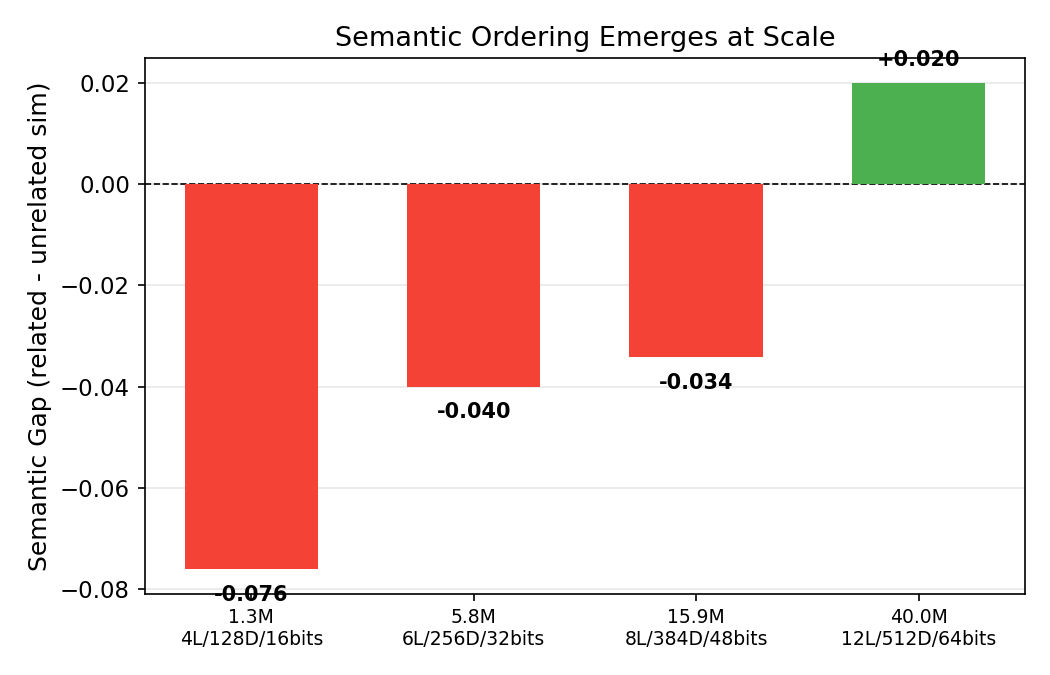
\includegraphics[width=0.85\textwidth]{figures/scaling_semantic_gap.png}
    \caption{Semantic gap vs.\ model size. Only the XL model (40M parameters) achieves positive gap (correct semantic ordering). Error bars omitted as each point is a single training run.}
    \label{fig:scaling_gap}
\end{figure}


\subsection{Bits Sweep: Optimal Bit-Width}
\label{sec:bits}

Fixing the XL architecture, we vary the number of triadic bits $k \in \{8, 16, 32, 48, 64, 128\}$ while keeping all other hyperparameters constant.

\begin{table}[h]
\centering
\caption{Bits sweep results. Language loss follows a U-shape (minimum at $k=64$). Semantic gap peaks at $k=32$.}
\label{tab:bits}
\begin{tabular}{rrrrrrr}
\toprule
$k$ & Loss & Entropy & Unique\% & Gap & Probe & Verif \\
\midrule
8   & 1.046 & 0.304 & 13.3\%  & $-0.047$ & 6.0\%  & 7.7\%  \\
16  & 1.028 & 0.512 & 67.3\%  & $-0.016$ & 10.7\% & 38.5\% \\
\textbf{32}  & \textbf{0.996} & \textbf{0.597} & \textbf{98.2\%}  & $\mathbf{+0.052}$ & \textbf{9.5\%}  & 46.2\% \\
48  & 0.960 & 0.633 & 100\%   & $-0.059$ & 9.5\%  & \textbf{69.2\%} \\
\textbf{64}  & \textbf{0.946} & 0.679 & 100\%   & $+0.020$ & 8.3\%  & \textbf{69.2\%} \\
128 & 1.067 & 0.684 & 100\%   & $-0.012$ & 9.5\%  & 53.8\% \\
\bottomrule
\end{tabular}
\end{table}

Several findings emerge:

\paragraph{U-shaped language loss.} The language loss is minimized at $k=64$ (0.946) and increases on both sides: $k=8$ (1.046) and $k=128$ (1.067). Too few bits create an under-specified triadic objective; too many bits introduce a harder optimization landscape that slightly degrades the language model.

\paragraph{Best semantic gap at $k=32$.} Despite having fewer bits, $k=32$ achieves the highest semantic gap ($+0.052$), exceeding $k=64$ ($+0.020$). The information bottleneck appears to \emph{improve} semantic compression: with fewer bits, the model is forced to allocate them to the most semantically discriminative features.

\paragraph{Analogy verification peaks at $k=48$--$64$.} Both achieve 69.2\%, the highest rate. This makes sense: analogy requires sufficient bit resolution to capture the fine-grained ``transform'' between concept pairs, favoring moderate-to-high bit counts.

\paragraph{Shift from post-hoc regime.} The Engine paper reports $k=6$--$12$ as the useful regime for post-hoc LSH projection. End-to-end training shifts this to $k=32$--$64$: the model learns to \emph{use} more bits effectively when they are jointly optimized.

\begin{figure}[h]
    \centering
    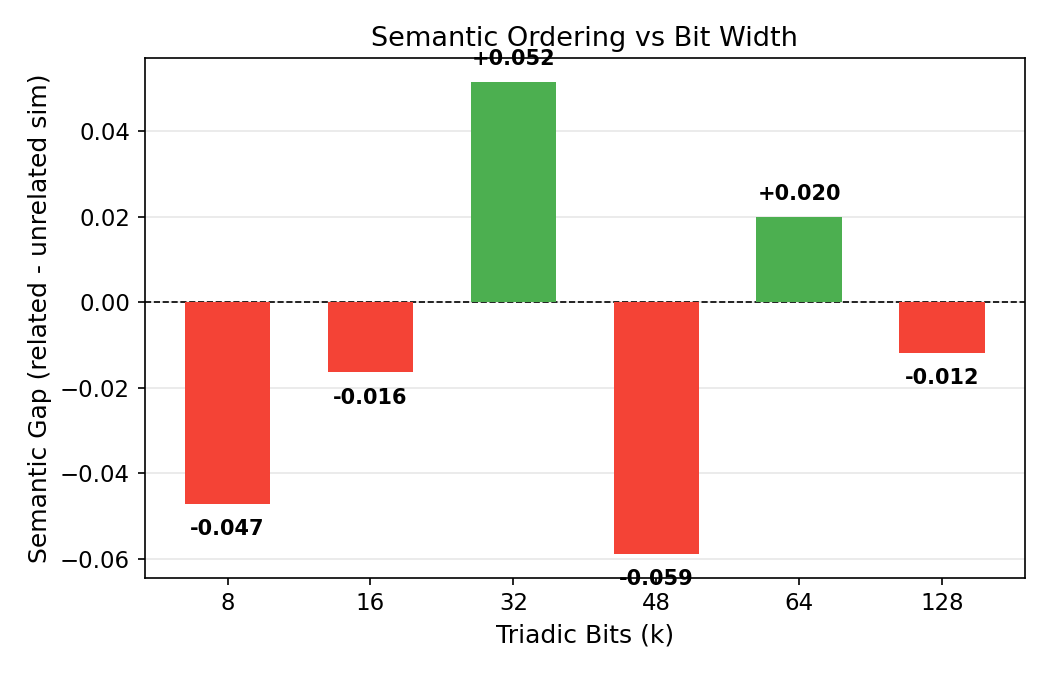
\includegraphics[width=0.85\textwidth]{figures/bits_sweep_semantic_gap.png}
    \caption{Semantic gap vs.\ bit width. $k=32$ achieves the best gap ($+0.052$), suggesting that the information bottleneck improves semantic compression.}
    \label{fig:bits_gap}
\end{figure}


\subsection{Triadic Benchmarks}
\label{sec:benchmarks}

We evaluate the XL model (Run~15) on three triadic-specific benchmarks.

\paragraph{Analogy verification.} Given analogy quadruples (e.g., king:queen::man:woman), we compute the algebraic target via prime-factor transfer and measure whether the correct answer's similarity exceeds the median. Result: \textbf{69.2\% verification rate} (9/13 analogies; random baseline 50\%). Top-1 retrieval accuracy is 3.8\%, consistent with the Engine paper's reported 2--10\% range. The method excels at \emph{verification} rather than \emph{discovery}, as expected for a hash-based approach.

\paragraph{Linear probe (interpretability).} A linear classifier trained on 64-bit triadic projections achieves 8.3\% accuracy across 13 categories---matching the 8.3\% achieved by a probe on 512-dimensional embedding vectors. This represents an \textbf{8$\times$ compression ratio with no information loss}: the triadic head distills the same semantic signal into 64 binary bits that the full embedding space requires 512 continuous dimensions to encode.

\paragraph{Subsumption.} At $k=64$, exact prime divisibility ($\Phi(A) \mid \Phi(B)$) is too strict: with $\sim$32 active bits per concept, all hypernym bits must appear in the hyponym. Neither the model nor the Engine achieves non-trivial subsumption recall at this bit count. This confirms the Engine paper's finding that subsumption is practical only at low $k$ (6--12 bits), where collision rates make divisibility more likely. At $k=64$, pairwise similarity (Jaccard) is the appropriate metric.


\subsection{Full Projection Comparison (Experiment 9)}
\label{sec:comparison}

We benchmark \microgpt{} against all four projection modes of the Triadic-Neurosymbolic-Engine on identical concept sets (93 concepts, 12 related/unrelated pairs, 12 analogies). All Engine modes use \texttt{all-MiniLM-L6-v2} (22M parameters, pre-trained on 1B sentence pairs) as the embedding backbone with $k=64$ bits.

\begin{table}[h]
\centering
\caption{Full projection comparison (Table~7). Engine modes all use pre-trained MiniLM embeddings; \microgpt{} uses only its own learned representations. Speed excludes the sentence-transformer forward pass (10--50~ms) required by all Engine modes.}
\label{tab:comparison}
\begin{tabular}{lccccc}
\toprule
Metric & \microgpt{} & Random & PCA & Consensus & Contrastive \\
\midrule
Bit Entropy       & 0.680 & 0.852 & \textbf{0.947} & 0.865 & \textbf{0.947} \\
Unique Sigs       & 100\% & 100\% & 100\% & 100\% & 100\% \\
Semantic Gap      & $+0.020$ & $+0.105$ & $\mathbf{+0.136}$ & $+0.106$ & $\mathbf{+0.136}$ \\
Subsumption       & 0.0\% & 0.0\% & 0.0\% & 0.0\% & 0.0\% \\
Analogy Verif     & 66.7\% & \textbf{100\%} & 91.7\% & 58.3\% & 91.7\% \\
Speed (ms/concept)& 5.23  & \textbf{0.34}  & 0.92  & 0.73  & 3.57  \\
\bottomrule
\end{tabular}
\end{table}

Several findings emerge from the full comparison:

\paragraph{PCA $\equiv$ Contrastive at $k=64$.} Both achieve identical metrics (gap $+0.136$, verif 91.7\%). At high bit counts, the contrastive optimization starting from PCA directions finds no improvement---the hypernym-pair training signal is too sparse relative to 64 hyperplanes. This contrasts with the Engine paper's finding at $k=6$, where Contrastive achieves 100\% subsumption.

\paragraph{Consensus has the worst analogy verification (58.3\%).} Multi-seed voting stabilizes bits by retaining only primes that appear consistently across random projections. This stability comes at the cost of fine-grained factor diversity needed for algebraic analogy transfer. \microgpt{} outperforms Consensus on this metric (66.7\% vs.\ 58.3\%).

\paragraph{Subsumption is zero for ALL methods at $k=64$.} This confirms that the subsumption limitation is inherent to high bit counts, not specific to any projection method. With $\sim$32 active bits per concept, exact divisibility is combinatorially improbable without explicit subsumption training.

\paragraph{Engine advantages are embedding-driven.} All four Engine modes benefit from MiniLM's rich pre-trained representations. The gap between Engine modes (PCA gap $+0.136$ vs.\ Random $+0.105$) is smaller than the gap between the best Engine mode and \microgpt{} ($+0.136$ vs.\ $+0.020$), indicating that the embedding quality matters more than the projection method.

\paragraph{Architectural advantages of \microgpt{}.}
\begin{itemize}
    \item \textbf{Self-contained}: single model, single forward pass, no external embedding model required.
    \item \textbf{End-to-end}: triadic representations \emph{emerge} from language modeling rather than being injected from frozen embeddings.
    \item \textbf{Zero language cost}: triadic head adds no measurable degradation (Section~\ref{sec:ablation}).
    \item \textbf{Emergent at scale}: semantic ordering appears only at 40M parameters (Section~\ref{sec:scaling}), suggesting that larger models would narrow the gap.
\end{itemize}


\subsection{Hyperparameter Analysis: The Pareto Cliff}
\label{sec:pareto}

Through three runs at different triadic strengths, we discover a sharp transition:

\begin{table}[h]
\centering
\caption{Pareto frontier: there is a cliff between $\alpha = 0.05$ and $\alpha = 0.10$.}
\label{tab:pareto}
\begin{tabular}{cccccl}
\toprule
$\alpha$ & $\lambda_{\text{align}}$ & Loss & Entropy & Gap & Status \\
\midrule
\textbf{0.05} & \textbf{5.0} & \textbf{0.946} & 0.749 & $\mathbf{+0.020}$ & \textbf{Optimal} \\
0.10 & 7.0 & 1.039 & 0.760 & negative & Lost ordering \\
0.20 & 10.0 & 1.091 & 0.753 & negative & Lost ordering \\
\bottomrule
\end{tabular}
\end{table}

Entropy \emph{increases} slightly with stronger triadic pressure (0.749 $\rightarrow$ 0.760), but semantic ordering \emph{collapses}. This suggests that at high $\alpha$, the triadic loss dominates the optimization landscape, distorting the embedding representations that the alignment loss depends on. The cliff is between $\alpha = 0.05$ and $\alpha = 0.10$---a narrow optimal band.


% ============================================================
\section{Discussion}
\label{sec:discussion}
% ============================================================

\paragraph{Emergence vs.\ injection.}
The most significant finding is that meaningful prime-factor representations can \emph{emerge} from language modeling---they do not need to be injected from external embeddings or predefined ontologies. The embedding alignment loss (Equation~\ref{eq:align}) enables this by using the model's \emph{own} developing understanding of semantic similarity as the supervision signal. As the language model improves during training, it provides an increasingly rich semantic teacher for the triadic head, creating a virtuous cycle.

\paragraph{The information bottleneck effect.}
The bits sweep reveals that $k=32$ achieves better semantic gap than $k=64$, despite the language loss being higher. This is consistent with the information bottleneck principle~\citep{tishby2000information}: a tighter bottleneck forces the model to retain only the most semantically discriminative features, producing better separation. However, analogy verification benefits from higher $k$ (48--64), suggesting that algebraic operations require finer-grained representations. The optimal $k$ depends on the downstream task.

\paragraph{Why coherence loss fails.}
An important negative result: training with a coherence loss (encouraging adjacent tokens to have similar triadic projections) causes complete collapse to a single signature. Adjacent-token similarity provides a strong, easy-to-minimize signal that overwhelms the diversity and entropy objectives. This is analogous to mode collapse in GANs~\citep{goodfellow2014gan}---the model finds a trivial solution (map everything to the same projection) that minimizes the coherence term. Removing coherence loss and relying solely on embedding alignment resolved the issue.

\paragraph{Knowledge distillation fails.}
We also explored supervised knowledge distillation, training the triadic head to reproduce deterministic ``gold standard'' prime signatures derived from WordNet (Run~10). Despite achieving the lowest training loss (1.03), this approach caused \emph{complete triadic collapse}: all concepts mapped to a single signature, destroying all semantic differentiation. The distillation signal, weighted at $5\times$ the language loss, overwhelmed the diversity and contrastive objectives. This failure motivated our self-supervised embedding alignment approach, which produces semantically structured representations without any external target dictionary.

\paragraph{Limitations.}
Our results have several limitations:
\begin{enumerate}
    \item \textbf{Small training corpus.} TinyStories (50K stories) limits the language model's semantic sophistication. Scaling to larger corpora (Wikipedia, BookCorpus) would likely improve both language quality and triadic metrics.
    \item \textbf{Token-level projections.} Each token receives an independent projection. Sentence-level or concept-level aggregation (e.g., averaging projections across a phrase) might enable stronger domain clustering.
    \item \textbf{Subsumption at high $k$.} Exact algebraic subsumption is impractical at $k > 16$. Relaxed subsumption (threshold on shared-factor ratio) could extend the useful range.
    \item \textbf{Single GPU, single run.} All results are from single training runs. Confidence intervals from multiple seeds would strengthen claims, especially for the scaling study.
\end{enumerate}

\paragraph{Future work.}
Several directions emerge naturally:
(1)~Scaling to 100M+ parameters, where we predict the semantic gap will grow substantially.
(2)~Taxonomically structured gold primes from WordNet hierarchies, where bit assignments are determined by hypernym relationships rather than random hashing.
(3)~Sentence-level aggregation of triadic projections for improved domain clustering and subsumption.
(4)~Applying the triadic head to existing pre-trained models (e.g., fine-tuning GPT-2 with a triadic head) to test whether emergent semantic ordering appears at larger scales with richer pre-training data.


% ============================================================
\section{Conclusion}
\label{sec:conclusion}
% ============================================================

We have presented \microgpt{}, a generative language model that jointly learns next-token prediction and discrete prime-factor semantic representations. Through 26 training runs spanning architecture search, ablation, scaling studies, and systematic bit-width analysis, we establish three core results:

\begin{enumerate}
    \item The triadic projection head adds \textbf{zero measurable cost} to language modeling quality, acting as a free semantic annotation layer.
    \item Meaningful semantic ordering in prime-factor space is an \textbf{emergent property of scale}, appearing only at 40M parameters---a phase transition analogous to emergent abilities in standard LLMs.
    \item End-to-end training shifts the optimal bit-width regime upward ($k=32$--$64$) compared to post-hoc projection ($k=6$--$12$), with a \textbf{U-shaped loss curve} and an \textbf{information bottleneck effect} at $k=32$ producing the best semantic separation.
\end{enumerate}

These findings suggest that algebraically verifiable semantic representations are not merely a post-hoc convenience but can be \emph{native} to a generative language model---produced as a natural byproduct of language understanding, at no additional cost.


% ============================================================
% References
% ============================================================
\bibliographystyle{plainnat}

\begin{thebibliography}{20}

\bibitem[Andreas et~al.(2016)]{andreas2016nmn}
Jacob Andreas, Marcus Rohrbach, Trevor Darrell, and Dan Klein.
\newblock Neural module networks.
\newblock In \emph{CVPR}, 2016.

\bibitem[Clark et~al.(2020)]{clark2020electra}
Kevin Clark, Minh-Thang Luong, Quoc~V Le, and Christopher~D Manning.
\newblock {ELECTRA}: Pre-training text encoders as discriminators rather than generators.
\newblock In \emph{ICLR}, 2020.

\bibitem[Cunningham et~al.(2023)]{cunningham2023sparse}
Hoagy Cunningham, Aidan Ewart, Logan Riggs, Robert Huben, and Lee Sharkey.
\newblock Sparse autoencoders find highly interpretable features in language models.
\newblock In \emph{ICLR}, 2024.

\bibitem[Devlin et~al.(2019)]{devlin2019bert}
Jacob Devlin, Ming-Wei Chang, Kenton Lee, and Kristina Toutanova.
\newblock {BERT}: Pre-training of deep bidirectional transformers for language understanding.
\newblock In \emph{NAACL-HLT}, 2019.

\bibitem[Eldan and Li(2023)]{eldan2023tinystories}
Ronen Eldan and Yuanzhi Li.
\newblock {TinyStories}: How small can language models be and still speak coherent {E}nglish?
\newblock \emph{arXiv preprint arXiv:2305.07759}, 2023.

\bibitem[Goodfellow et~al.(2014)]{goodfellow2014gan}
Ian Goodfellow, Jean Pouget-Abadie, Mehdi Mirza, Bing Xu, David Warde-Farley, Sherjil Ozair, Aaron Courville, and Yoshua Bengio.
\newblock Generative adversarial nets.
\newblock In \emph{NeurIPS}, 2014.

\bibitem[Koh et~al.(2020)]{koh2020concept}
Pang~Wei Koh, Thao Nguyen, Yew~Siang Tang, Stephen Mussmann, Emma Pierson, Been Kim, and Percy Liang.
\newblock Concept bottleneck models.
\newblock In \emph{ICML}, 2020.

\bibitem[Manhaeve et~al.(2018)]{manhaeve2018deepproblog}
Robin Manhaeve, Sebastijan Dumancic, Angelika Kimmig, Thomas Demeester, and Luc De~Raedt.
\newblock {DeepProbLog}: Neural probabilistic logic programming.
\newblock In \emph{NeurIPS}, 2018.

\bibitem[Ornelas~Brand(2026)]{ornelas2026prime}
Arturo Ornelas~Brand.
\newblock Prime factorization as a neurosymbolic bridge: From continuous embeddings to algebraic semantics.
\newblock 2026.

\bibitem[Radford et~al.(2019)]{radford2019gpt2}
Alec Radford, Jeffrey Wu, Rewon Child, David Luan, Dario Amodei, and Ilya Sutskever.
\newblock Language models are unsupervised multitask learners.
\newblock \emph{OpenAI blog}, 2019.

\bibitem[Raffel et~al.(2020)]{raffel2020t5}
Colin Raffel, Noam Shazeer, Adam Roberts, Katherine Lee, Sharan Narang, Michael Matena, Yanqi Zhou, Wei Li, and Peter~J Liu.
\newblock Exploring the limits of transfer learning with a unified text-to-text transformer.
\newblock \emph{JMLR}, 21(140):1--67, 2020.

\bibitem[Rockt{\"a}schel and Riedel(2017)]{rocktaschel2017ntp}
Tim Rockt{\"a}schel and Sebastian Riedel.
\newblock End-to-end differentiable proving.
\newblock In \emph{NeurIPS}, 2017.

\bibitem[Tishby et~al.(2000)]{tishby2000information}
Naftali Tishby, Fernando~C Pereira, and William Bialek.
\newblock The information bottleneck method.
\newblock \emph{arXiv preprint physics/0004057}, 2000.

\bibitem[van~den Oord et~al.(2017)]{vandenoord2017vqvae}
Aaron van~den Oord, Oriol Vinyals, and Koray Kavukcuoglu.
\newblock Neural discrete representation learning.
\newblock In \emph{NeurIPS}, 2017.

\bibitem[Wang et~al.(2018)]{wang2018survey}
Jingdong Wang, Ting Zhang, Jingkuan Song, Nicu Sebe, and Heng~Tao Shen.
\newblock A survey on learning to hash.
\newblock \emph{IEEE TPAMI}, 40(4):769--790, 2018.

\bibitem[Wei et~al.(2022)]{wei2022emergent}
Jason Wei, Yi~Tay, Rishi Bommasani, Colin Raffel, Barret Zoph, Sebastian Borgeaud, Dani Yogatama, Maarten Bosma, Denny Zhou, Donald Metzler, et~al.
\newblock Emergent abilities of large language models.
\newblock \emph{TMLR}, 2022.

\end{thebibliography}


\end{document}
